% arara: pdflatex
% arara: biber
% arara: makeindex
% arara: nomencl
% arara: pdflatex
% arara: pdflatex

\documentclass[a4paper,12pt]{article}
%\RequirePackage[l2tabu,orthodox]{nag}

\usepackage{upreport}
\usepackage{tabularx}
\usepackage{amssymb}
\usepackage{siunitx}
\addbibresource{report.bib}
\title{Project Model}
\subject{CBT 700}
\date{\today}

%Nomenclature unit command
\newcommand{\nomunit}[1]{%
\renewcommand{\nomentryend}{\hspace*{\fill}#1}}

% Create a custom user command or run the following 
%  makeindex %.nlo -s nomencl.ist -o %.nls
% execute this command after compiling your file once, then compile a second time to generate a nomenclature table



\begin{document}


\section{System Diagram}

The Process Floe Diagram of the system, with all the relevant inputs, outputs and disturbances are displayed in Figure~\ref{fig:processpfd}.

\begin{figure}[tbph]
	\centering
	\label{fig:processpfd}
	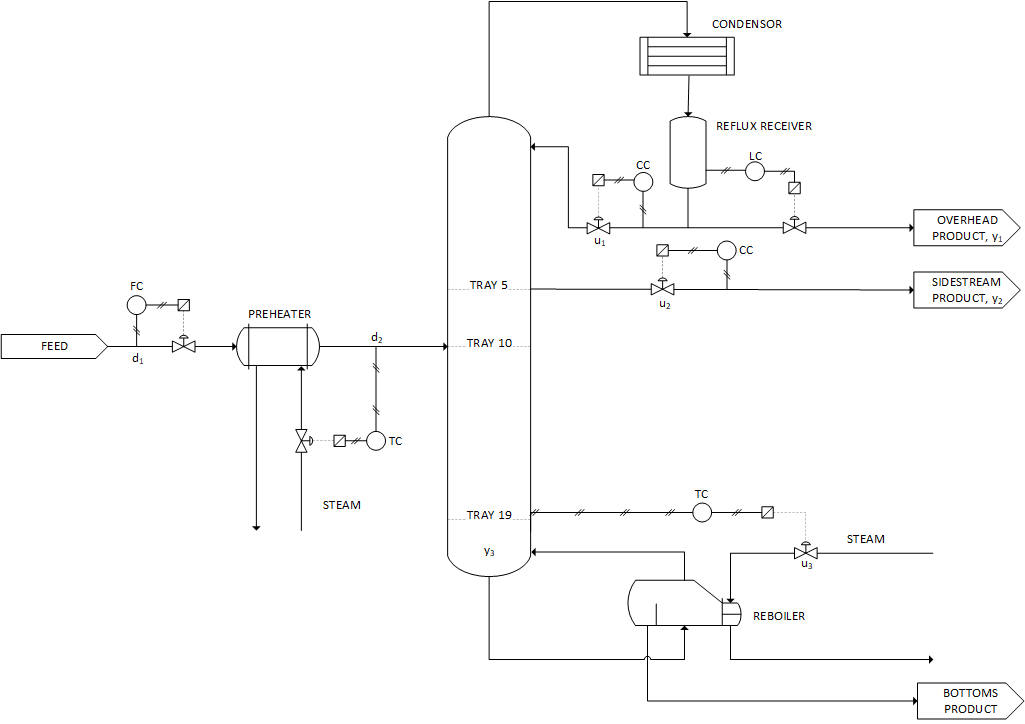
\includegraphics[width=0.9\linewidth]{../Process_PFD}
	\caption{Process flow diagram of the system}
\end{figure}

\newpage
\section{System Description}

\newpage
\section{System Variables}

\begin{table}[h]
	\label{teb:Variables}
	\centering
	\caption{Summary of all the model variables.}
	\begin{tabular}{cccc}
		\hline
		\multicolumn{4}{c}{Input Variables}                                       \\
		
		Variable & Description                       & Steady State Value & Units \\
		\hline
		$u_1$       & Reflux flow rate                  & 0.18               & gpm   \\
		$u_2$       & Side stream product flow rate     & 0.046              & gpm   \\
		$u_3$       & Reboiler steam pressure           & 20                 & psi   \\
		\hline
		\multicolumn{4}{c}{Output Variables}                                      \\
		
		Variable & Description                       & Steady State Value & Units \\
		\hline
		$y_1$       & Overhead ethanol mole fraction    & 0.7                & -     \\
		$y_2$       & Side stream ethanol mole fraction & 0.52               & -     \\
		$y_3$       & Tray \#19 temperature             & 92                 & \si{\celsius} \\
		\hline
		\multicolumn{4}{c}{Disturbance Variables}                                 \\
		
		Variable & Description                       & Steady State Value & Units \\
		\hline
		$d_1$       & Feed flow rate                    & 0.8                & gpm   \\
		$d_2$       & Feed temperature                  & 78                 & \si{\celsius} \\\hline
	\end{tabular}
\end{table}

\newpage
\section{System Model}

The model takes the form of a commonly employed linear model for a MIMO system,

\begin{equation}
\textbf{y}(s) = \textbf{G}(s)\textbf{u}(s) + \textbf{G}_{d}(s)\textbf{d}(s)
\end{equation}

where

\begin{equation}
	\textbf{G}(s) = \begin{bmatrix}
	G_{11} & G_{12} & G_{13} \\
	G_{21} & G_{22} & G_{23} \\
	G_{31} & G_{32} & G_{33} \\
	\end{bmatrix} = \begin{bmatrix}
	\frac{0.66e^{-2.6s}}{6.7s+1} & \frac{-0.61e^{-3.5s}}{8.64s+1} & \frac{-0.0049e^{-s}}{9.06s+1} \\
	\frac{1.11e^{-6.5s}}{3.25s+1} & \frac{-2.36e^{-3s}}{5.0s+1} & \frac{-0.012e^{-1.2s}}{7.09s+1} \\
	\frac{-34.68e^{-9.2s}}{8.15s+1} & \frac{46.2e^{-9.4s}}{10.9s+1} & \frac{0.87(11.61s+1)e^{-s}}{(3.89s+1)(18.8s+1)}
	\end{bmatrix}
\end{equation}

and

\begin{equation}
\textbf{G}_{d}(s) = \begin{bmatrix}
G_{d11} & G_{d12} \\
G_{d21} & G_{d22} \\
G_{d31} & G_{d32} \\
\end{bmatrix} = \begin{bmatrix}
\frac{0.14e^{-12s}}{6.2s+1} & \frac{-0.0011(26.32s+1)e^{-2.66s}}{(7.85s+1)(4.63s+1)} \\
\frac{0.53e^{-10.5s}}{6.9s+1} & \frac{-0.0032(19.62s+1)e^{-3.44s}}{(7.29s+1)(8.94s+1)} \\
\frac{-11.54e^{-0.6s}}{7.01s+1} & \frac{0.32e^{-2.6s}}{7.76s+1}
\end{bmatrix}
\end{equation}


\appendix
\renewcommand{\thefigure}{\thesection.\arabic{figure}}
\renewcommand{\thetable}{\thesection.\arabic{table}}
\renewcommand{\thepage}{\thesection.\arabic{page}}
\end{document}